% 3.3.1 Diseño con el usuario (T2): prototipo visual sobre los mockups del Obj. 2 y ajustes pedidos por el personal.

\subsubsection{Diseño con el usuario}

El prototipo visual, construido en HTML, aplica la paleta sobre los mockups (Figuras~\ref{fig:ob2_mockup_agenda} y \ref{fig:ob2_mockup_atencion}) y se revisó con el personal antes de construir cada pantalla.

La agenda de la secretaria (Figura~\ref{fig:ob3_proto_agenda}) muestra una columna por profesional y el estado de cada cita, incluidas las del agente (RF07).

\begin{figure}[H]
\centering
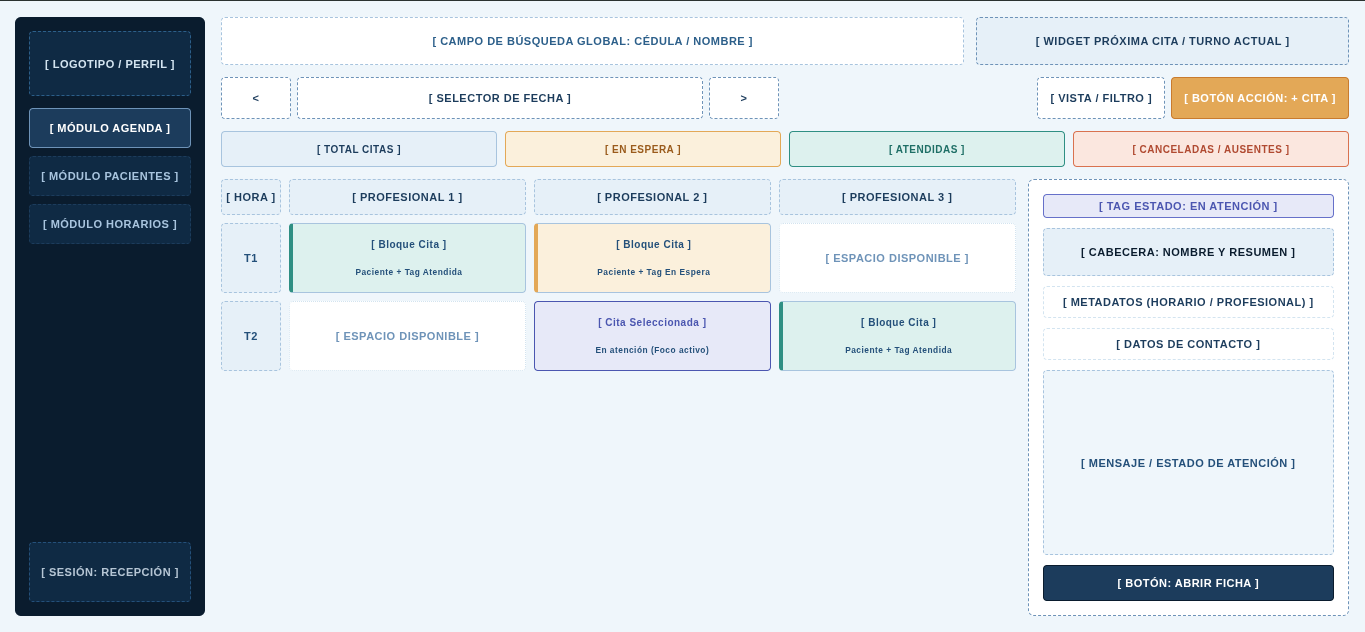
\includegraphics[width=\linewidth]{img/Objetivo3/Wireframe_Agenda_Secretaria.png}
\caption{Prototipo de la agenda de la secretaria}
\label{fig:ob3_proto_agenda}
\end{figure}

La ficha de recepción (Figura~\ref{fig:ob3_proto_recepcion}) reúne las citas y el estado de cuenta, sin datos clínicos (RF08, RNF01).

\begin{figure}[H]
\centering
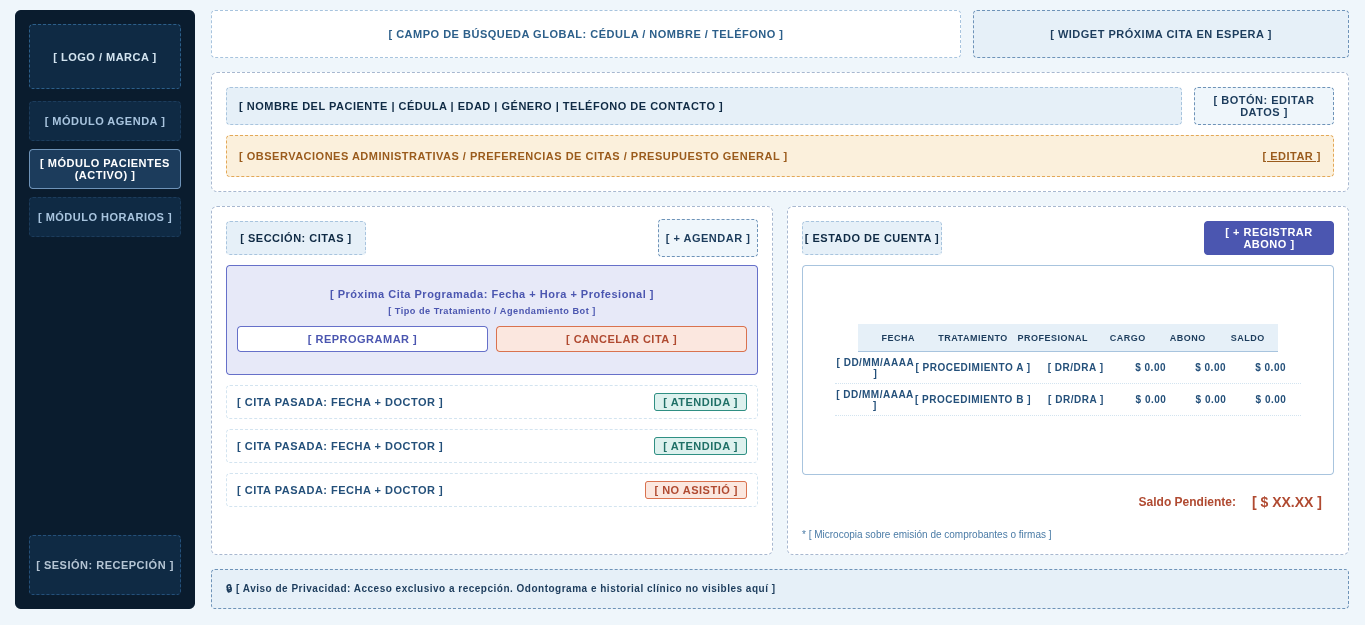
\includegraphics[width=\linewidth]{img/Objetivo3/Wireframe_Atencion_Secretaria.png}
\caption{Prototipo de la ficha de recepción: citas y estado de cuenta del paciente}
\label{fig:ob3_proto_recepcion}
\end{figure}

El odontólogo ve sus citas en un tablero por estado y abre la atención con cita o sin ella (Figura~\ref{fig:ob3_proto_citas}; RF06).

\begin{figure}[H]
\centering
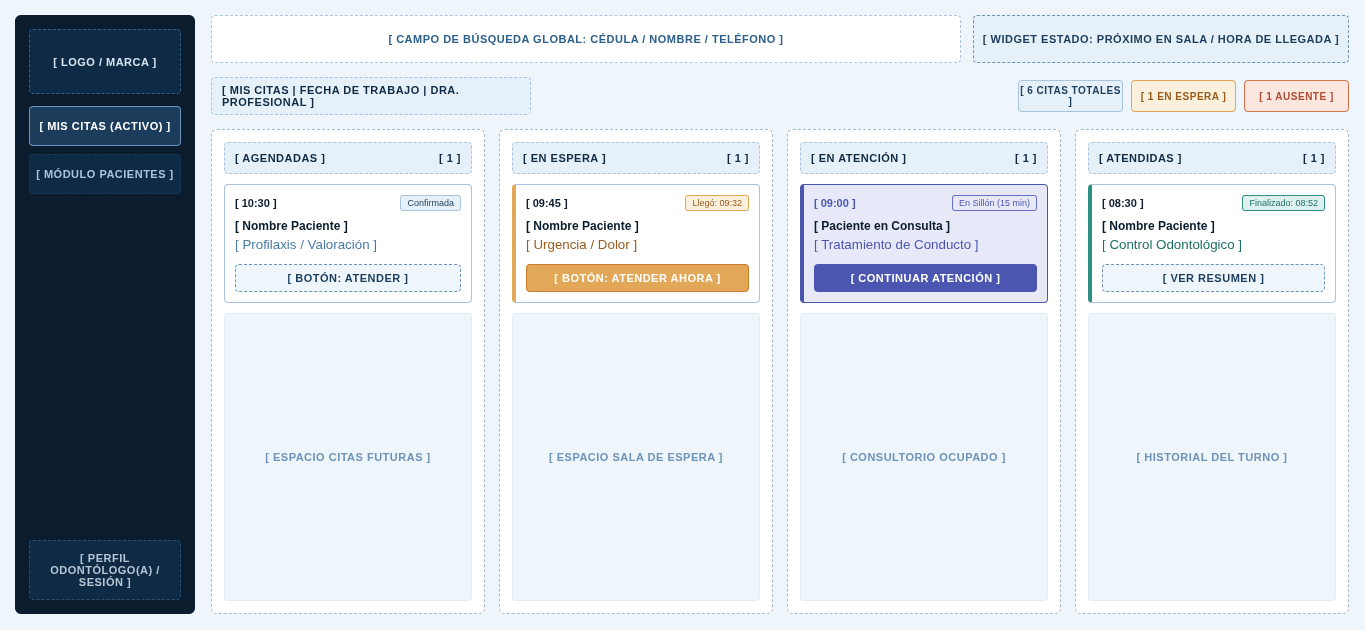
\includegraphics[width=\linewidth]{img/Objetivo3/Wireframe_Citas_Odontologo.png}
\caption{Prototipo de las citas del odontólogo}
\label{fig:ob3_proto_citas}
\end{figure}

La atención reúne las alertas clínicas y el odontograma por pieza y cara, en rojo lo pendiente y en azul lo realizado (Figura~\ref{fig:ob3_proto_atencion}; RF02, RNF06).

\begin{figure}[H]
\centering
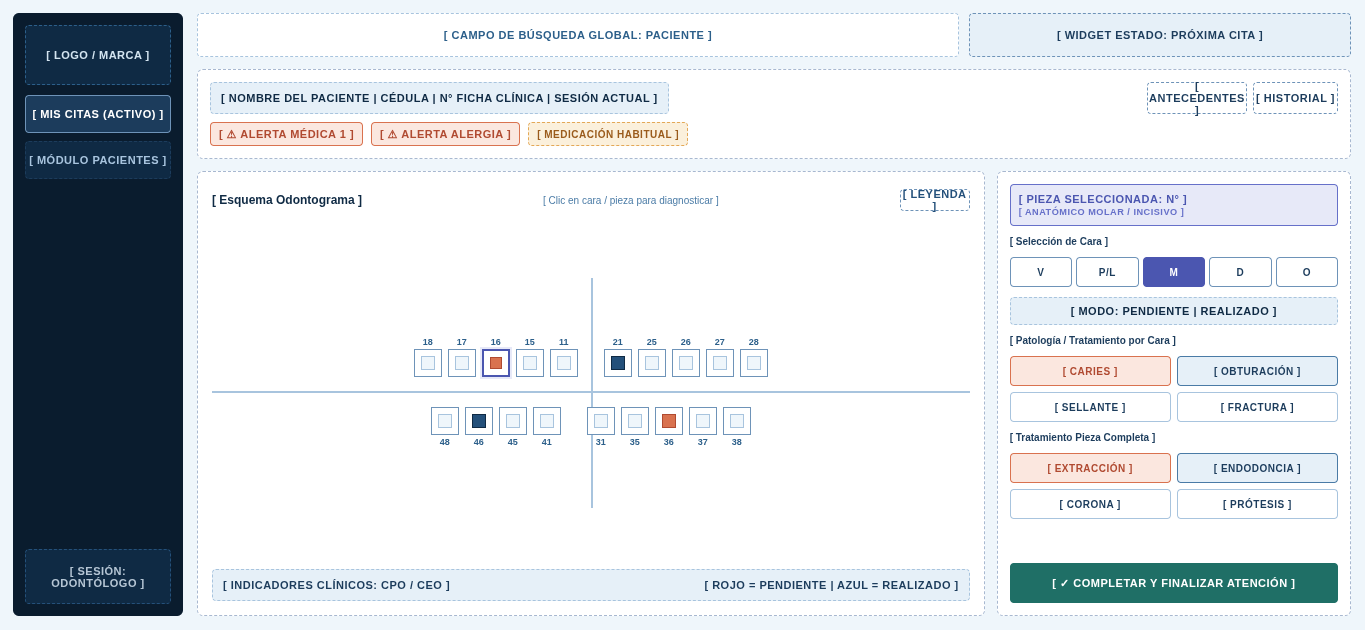
\includegraphics[width=\linewidth]{img/Objetivo3/Wireframe_Atencion_Odontologo.png}
\caption{Prototipo de la atención del odontólogo con el odontograma}
\label{fig:ob3_proto_atencion}
\end{figure}

La Tabla~\ref{tab:ob3_ajustes} resume las observaciones del personal y el ajuste incorporado en la construcción.

% CONFIRMAR con el autor qué observaciones vinieron del personal
% (fuente: bellidental-frontend/docs/IMPLEMENTATION-PLAN.md §5.22-5.24).
\begingroup
\fontsize{9}{11}\selectfont
\renewcommand{\arraystretch}{1.2}
\setlength{\LTpre}{0pt}\setlength{\LTpost}{6pt}
\setlength{\tabcolsep}{4pt}
\begin{xltabular}{\linewidth}{|>{\raggedright\arraybackslash}p{2.0cm}|>{\raggedright\arraybackslash}X|>{\raggedright\arraybackslash}X|>{\raggedright\arraybackslash}p{1.8cm}|}
\caption{Observaciones del personal y ajustes al prototipo}
\label{tab:ob3_ajustes} \\
\hline
\textbf{Perfil} & \textbf{Observación} & \textbf{Ajuste} & \textbf{Req.} \\ \hline
\endfirsthead
\hline
\textbf{Perfil} & \textbf{Observación} & \textbf{Ajuste} & \textbf{Req.} \\ \hline
\endhead
Odontólogo & Faltan medicamentos y posologías en el catálogo & Catálogo administrable, también desde la receta & RF04, RF05 \\ \hline
Odontólogo & Los formularios tapan el odontograma & Tratamientos y receta en un panel lateral & RNF06 \\ \hline
Secretaria & El paciente sin cita espera un horario libre & Horarios de hoy en bloques de 15 min desde la hora actual & RF07 \\ \hline
Director & Distinguir a cada profesional en la agenda & Color editable por profesional & RF07 \\ \hline
Todos & Ubicar pacientes atendidos o con saldo & Lista de pacientes con filtros de período y saldo & RF06, RF08 \\ \hline
\end{xltabular}
\endgroup
